
\REM{
\FDI\ is an \FDO\ inliner that can be parameterized, and it also employs the \CP\ methodology. To show that \FDI\ can active better results than well established static inliners, some experiments were designed. \FDI\ inliner is fully described in ~\cite{BerubePhD}. These experiments followed a single-run methodology, for the training phase and for the testing phase. The input set was defined as a minimal coverage set, and the training set was defined as the whole input set except for the input under test. The experiment compares the runtime performance of the programs when inlined by \llvm\ static inliner with the the performance of the same program when inlined by \FDI\ inliner. 

To make a fair comparison on the inliners and have a reasonable and short input set, some experimental decisions were taken. Both inliners were also evaluated with respect to the baseline Never, which means never inline. The input set for each program was defined to be representative for the entire set of inputs, and are described as follows. The input set for the programs \bzip, \gzip, \gobmk, and \gcc\ is a small subset of the original 15-input set described in \refSection{sec:description}. The results show a slight improvement over \llvm.


The \bzip\ and \gzip\ programs were executed using a representative set of inputs, where compression tasks and decompression tasks were tested under similar inputs.
The compression set contains the following inputs, with the compression level shown in parentheses:
\begin{itemize}

%\item {\tt avernum (-3)}: The installer for the demo version of the game  ``Avernum: Escape from the Pit'' from Spiderweb Software.

\item {\tt cards (-4)}: A collection of greeting card layouts in the TIFF (uncompressed) image format.

%\item {\tt ebooks (-5)}: A collection of ebooks, with and without images, and in a variety of formats, from Project Gutenberg\footnote{http://www.gutenberg.org}.

%\item {\tt potemkin-mp4 (-6)}: The 1925 movie ``Bronenosets Potyomkin (Battleship Potemkin)'' in MP4 format, from the Internet Archive\footnote{http://archive.org/details/BattleshipPotemkin}.

%\item {\tt proteins-1 (-7)}: A sample of 33 proteins from the RCSB Protein Data Bank database.  6 files for each protein, each stored in a different text-based format, provide different characteristics of the protein's structure\footnote{http://www.rcsb.org}.

\item {\tt revelation-ogg (-8)}: The audio book ``The Revelation of Saint John'' in OGG format, from Project Gutenberg\footnote{http://www.gutenberg.org/ebooks/22945}.

%\item {\tt usrlib-so (-9)}: A collection of shared object (.so) files from {\tt /usr/lib/} of a 32-bit gentoo-linux machine.

\end{itemize}

The decompression set for each compressor uses the same base set of files, pre-compressed by the appropriate compressor at the default compression level.  The decompression set is composed of:
\begin{itemize}
\item {\tt auriel}: The ``Auriel's Retreat'' land-mass addition mod by lance4791 for the game ``The Elder Scrolls IV: Oblivion'' from Bethesda Softworks\footnote{http://planetelderscrolls.gamespy.com/View.php?view=\\ \hspace*{150 pt}OblivionMods.Detail\&id=5949}.

%\item {\tt gcc-453}: The source-code archive of the \gcc\ compiler, version 4.5.3\footnote{http://gcc.gnu.org/gcc-4.5}.

%\item {\tt lib-a}: A collection of library files (.a) from {\tt /lib/} of a gentoo-linux machine.  As per the gentoo development guide, a library will be installed in {\tt /lib} (boot critical) or {\tt /usr/lib} (general applications), but not both\footnote{http://devmanual.gentoo.org/general-concepts/filesystem/index.html}.

%\item {\tt mohicans-ogv}: The 1920 movie ``Last of the Mohicans'' in OGV (ogg video) format, from the Internet Archive\footnote{http://archive.org/details/last\_of\_the\_mohicans\_1920}.

\item {\tt ocal-019}: The Open Clip Art Library archive, version 0.19. The images are primarily in vector-graphics formats\footnote{http://openclipart.org/collections}.

%\item {\tt paintings-jpg}: A collection of watercolor paintings, in JPG format.

\item {\tt proteins-2}: A completely different sample of 157 proteins from the RCSB Protein Data Bank database, each in 6 different file formats.

%\item {\tt sherlock-mp3}: The audio book ``The Adventures of Sherlock Holmes'' in MP3 format, from Project Gutenberg\footnote{http://www.gutenberg.org/ebooks/28733}.

\end{itemize}

%\subsection{Setting up the experiments}

%============ Hardware

The experiments were run on $20$ Dell Optiplex 755, whose characteristics are:
\begin{itemize}

\item Intel Duo Core E6750 2.66 GHz processor;

\item 4 GB RAM;

\item DVD-RW drive;

\item Intel Pro/1000 Gb ethernet;

\item Gigabyte GeForce 8600 video cards;

\item 250 GB SATA II drive. 

\end{itemize}
}

%============ Our results

This section presents an evaluation of the \FDI\  and the \llvm\ static inliner by comparing their performance against the baseline \Never.
The height of each bar in all graphs in this section represents a normalized running time that is the quotient between the running time of the inliner evaluated and the running time of \Never. Each execution time used in this calculation is the minimum of three executions of the same executable program with the same input. Therefore a normalized running time below one indicates better (faster) performance than \Never. The speedups in the tables in this section are calculated as the ratio between the execution times of \FDI\ and \llvm.%, hence, whenever the values are less than one then there is a speedup, otherwise a slowdown.

\subsection{Presenting the speedup results}
\label{sec:speedupresult}

The data points were selected as representing a single-run methodology for the experiments, and three benchmarks were used to test the hypotheses, \bzip, \gzip, and \gcc. The points selected were the best-run times for \FDI\ and the worst-run times for \llvm. The results are presented in the following way, \bzip\ and \gzip, are grouped, while \gcc\ is separately described in other section, because the program behavior is completely different from the other two benchmarks.

\subsubsection{Case Study 1 \gcc}

The results in \refTable{tab:speedupgcc} show that \FDI\ outperformed \llvm\ for all inputs for \gcc. The results are normalized by the baseline Never (no inlining) and the geometric mean of the
\FDI\  speedup over \llvm\ was $2.52 \%$  for \gcc\ with this set of inputs.


\begin{table}
  \centering
  \begin{tiny}
  
\begin{tabular}{lllll}

{\bf Input} & {\bf \FDO\ normalized} & {\bf \llvm\ normalized} & {\bf Speedup} \\ \hline

166 & 0.9532 & 0.9755 & 0.9771  \\
c-typeck & 0.9400 & 0.9845 & 0.9548  \\
Cp-decl & 0.9589 & 0.9784 & 0.9800  \\
expr & 0.9208 & 0.9567 & 0.9624  \\
expr2 & 0.9208 & 0.9686 & 0.9506  \\
g23 & 0.9860 & 1.0441 & 0.9443  \\
integrate & 0.9810 & 1.0000 & 0.9810  \\
s04 & 0.9987 & 1.0153 & 0.9836  \\
lbm-all & 0.9696 & 1.0303 & 0.9411  \\
mcf-all & 1.0000 & 1.0270 & 0.9736  \\  \hline
Geomean & & & 0.9630 \\
  
\hline
\end{tabular}

  \end{tiny}
  \caption{Execution times normalized by the execution time of \Never\ and \FDI\ speedup over \llvm\ for \gcc.}
  \label{tab:speedupgcc}
\end{table}

The \refFigure{fig:gccall} shows that the \FDI\ inliner outperforms Never and \llvm\ through all the inputs, which explains the speedup.


\REM{Nevertheless, this result can be improved by just selecting less inputs from the short input set applied without changing the set substantially. In this case the speedup reported is $4.56 \%$ over \llvm, as shown in \refTable{tab:speedupgcc1} and \refFigure{fig:speedupgcc1}.

\begin{table}
  \centering
  \begin{tiny}
  
\begin{tabular}{lllll}

{\bf Input} & {\bf \FDO\ normalized} & {\bf \llvm\ normalized} & {\bf Speedup} \\ \hline

c-typeck & 0.9097 & 0.9745 & 0.9335  \\
expr & 0.9035 & 0.9552 & 0.9458  \\
expr2 & 0.8630 & 0.9660 & 0.8934  \\
g23 & 0.9119 & 0.9849 & 0.9259  \\
lbm-all & 0.8888 & 1.0000 & 0.8888  \\
mcf-all & 0.9487 & 1.0000 & 0.9487  \\  \hline
Geomean & & & 0.9224 \\
  
\hline
\end{tabular}

  \end{tiny}
  \caption{Extract of the data collected during the experiment with \gcc}
  \label{tab:speedupgcc1}
\end{table}

\begin{figure}
  \centering
  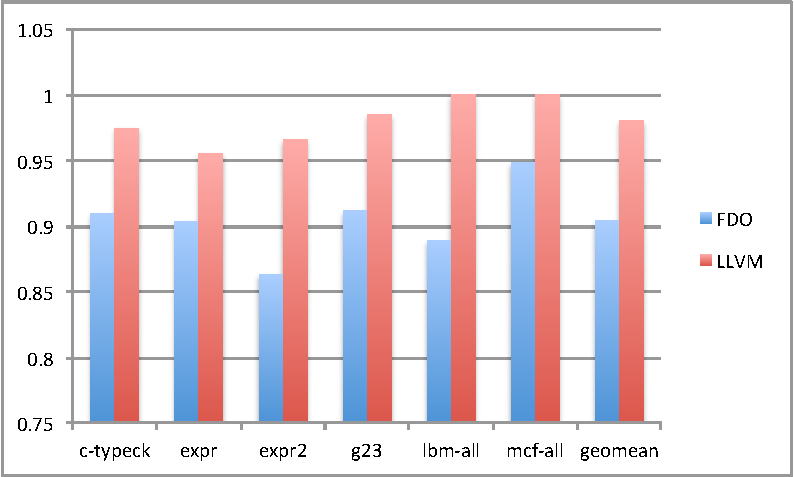
\includegraphics[width=1.00\linewidth]{Figures/speedupgcc1}
  \caption{Extract of the running times of the \gcc\ inlined versions, normalized by Never}
  \label{fig:speedupgcc1}
\end{figure}
}
\subsubsection{Case Study 2: \bzip\  and \gzip}

For the \bzip\ and \gzip\ cases, the experiments showed a slight speedup over \llvm. The data collected from the \bzip\ runs are summarized in \refTable{tab:speedupb}. In this table the speedup achieved was a slight one, $0.46 \%$ over \llvm\ results, and $0.71 \%$ over Never (no inlining), whereas \llvm\ achieved a speedup of $0.25 \%$ over Never.

\begin{table}
  \centering
  \begin{tiny}
  
\begin{tabular}{lllll}

{\bf Input} & {\bf \FDO\ time (sec)} & {\bf Never time (sec)} & {\bf \llvm\ time (sec)} & {\bf Speedup} \\ \hline

auriel & 7.66 & 7.88 & 7.94 & 0.9647   \\ 
cards & 29.52 & 29.79 & 29.76 & 0.9919  \\
ocal & 44.94 & 44.99 & 45.33 & 0.9913  \\ 
proteins-2 & 79.6 & 81.11 & 80.71 & 0.9862  \\
revelation & 5.24 & 5.31 & 5.25 & 0.9980  \\  \hline
Geomean & & & & 0.9864 \\
  
\hline
\end{tabular}

  \end{tiny}
  \caption{Summary of the data collected during the experiment with \bzip}
  \label{tab:speedupb}
\end{table}

\refFigure{fig:speedup} shows the running time normalized by the time of Never. And again the \FDI\ inliner outperforms Never and \llvm\ through all the inputs, the same way the former experiments did. %The experiment on the program \bzip\ shed some light on the use of inliners even considering such smaller programs, and these results can be fully explored in future research.

\begin{figure}
  \centering
  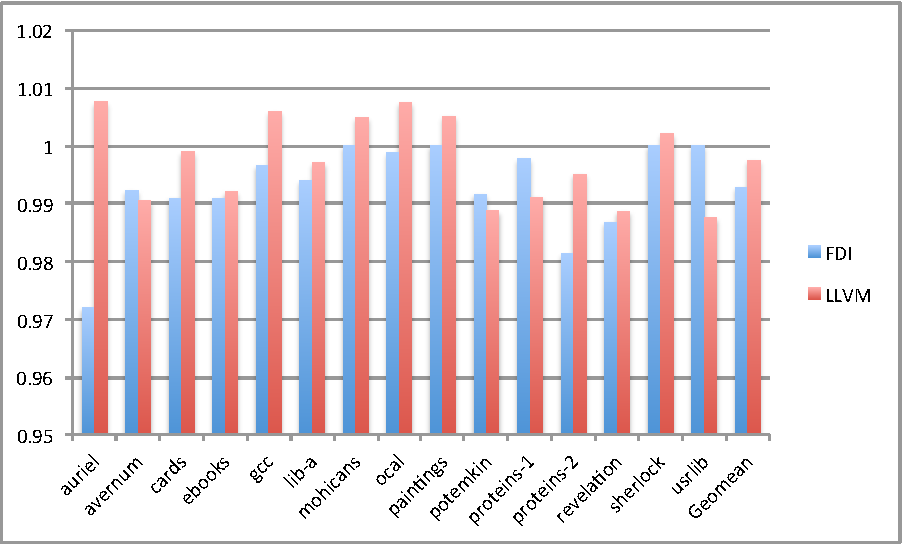
\includegraphics[width=1.00\linewidth]{Figures/speedupbzipall}
  \caption{Running times of the \bzip\ inlined versions, normalized by Never}
  \label{fig:speedup}
\end{figure}

The final result for the speedup, despite being a slight improvement, represents that the \FDI\ inliner can actually be employed instead of the \llvm\ inliner. And this result is also significant because the program \bzip\ is small, simple, and not particularly fitted to inlining, leading to a conjecture that \FDI\ inliner are better than static ones. Which opens a wide range of experiments with other programs to confirm this conjecture.

The experiment with \gzip\ was a starting point to test the conjecture, and the results are quite similar to those from \bzip, and confirmed a speedup of $2.26 \%$ over \llvm\ results, and a speedup of $2.90 \%$ over Never (no inlining) and \llvm\ got a speedup of $0.66 \%$ over Never. These results can be seen in \refTable{tab:speedupz}, where the times are already normalized by the baseline Never (no inlining). \refFigure{fig:speedupz} shows the normalized running time for \gzip, and it also outperforms Never and \llvm\ through all inputs.

\begin{table}
  \centering
  \begin{tiny}
  
\begin{tabular}{lllll}

{\bf Input} & {\bf \FDO\ normalized} & {\bf \llvm\ normalized} & {\bf Speedup} \\ \hline

auriel & 0.9924 & 0.9924 & 1.0000   \\ 
cards & 0.9801 & 1.0092 & 0.9712  \\
ocal & 0.9914 & 1.0122 & 0.9794  \\ 
proteins-2 & 0.9905 & 1.0094 & 0.9811  \\
revelation & 0.9708 & 1.0072 & 0.9637  \\  \hline
Geomean & & & 0.9790 \\
  
\hline
\end{tabular}

  \end{tiny}
  \caption{Summary of the data collected during the experiment with \gzip}
  \label{tab:speedupz}
\end{table}

\begin{figure}
  \centering
  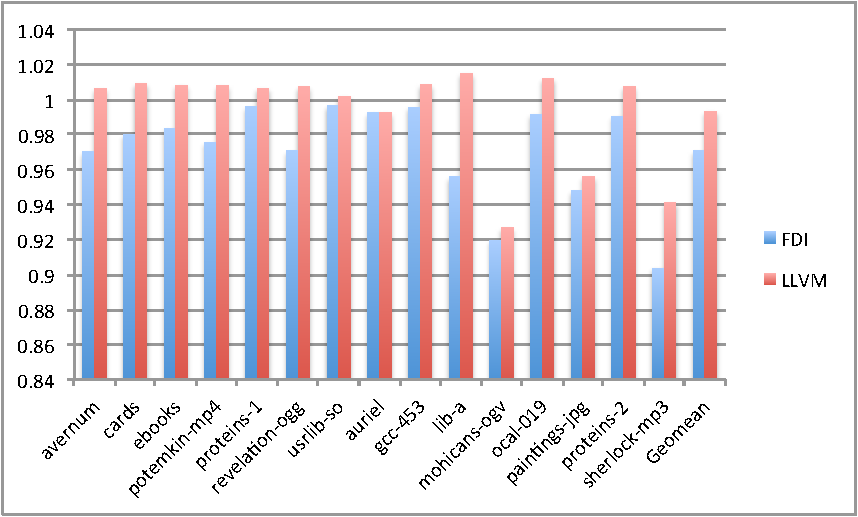
\includegraphics[width=1.00\linewidth]{Figures/speedupgzipall}
  \caption{Running times of the \gzip\ inlined versions, normalized by Never}
  \label{fig:speedupz}
\end{figure}

The results of the experiment are also consistent with other similar findings in the literature, whereas employing single-run experiments does not generate any kind of disturbance in the analysis, and the speedup result are statistically sound. So we can confirm a speedup over the static inliner for the \bzip\ and \gzip\ cases.

\subsubsection{Case Study 3 \gobmk}

For the \gobmk\ benchmark the results show a speedup of $1.01 \%$ over \llvm\, and a $0.99 \%$ speedup over Never, whereas \llvm\ had a $0.02 \%$ slowdown over Never, for the short input set used. This result is summarized in \refTable{tab:speedupgobmk}. The results are normalized by the baseline Never (no inlining).

\begin{table}
  \centering
  \begin{tiny}
  
\begin{tabular}{lllll}

{\bf Input} & {\bf \FDO\ normalized} & {\bf \llvm\ normalized} & {\bf Speedup} \\ \hline

13x13 & 0.9922 & 0.9983 & 0.62\%  \\
arb & 0.9939 & 0.9969 & 0.30\%  \\
arend & 0.9894 & 1.0017 & 1.23\%  \\
arion & 0.9934 & 0.9989 & 0.55\%  \\
atari\_atari & 0.9838 & 1.0000 & 1.61\%  \\
buzco & 0.9912 & 0.9970 & 0.58\%  \\
connect & 0.9881 & 1.0118 & 2.34\%  \\
connection & 0.9881 & 1.0039 & 1.57\%  \\
dniwog & 0.9924 & 0.9977 & 0.53\%  \\
nicklas2 & 0.9980 & 1.0019 & 0.39\%  \\
nicklas4 & 0.9896 & 0.9960 & 0.64\%  \\
nngs & 0.9905 & 0.9989 & 0.84\%  \\
score2 & 0.9775 & 0.9958 & 1.84\%  \\
trevorc & 0.9928 & 1.0004 & 0.76\%  \\
trevord & 0.9895 & 1.0025 & 1.30\%  \\  \hline

Geomean & & & 1.01\%  \\
  
\hline
\end{tabular}

  \end{tiny}
  \caption{Summary of the data collected during the experiment with \gobmk}
  \label{tab:speedupgobmk}
\end{table}

The \refFigure{fig:speedupgobmk} shows that the \FDI\ inliner outperforms Never and \llvm\ through all the inputs, which explains the speedup.

\begin{figure}
  \centering
  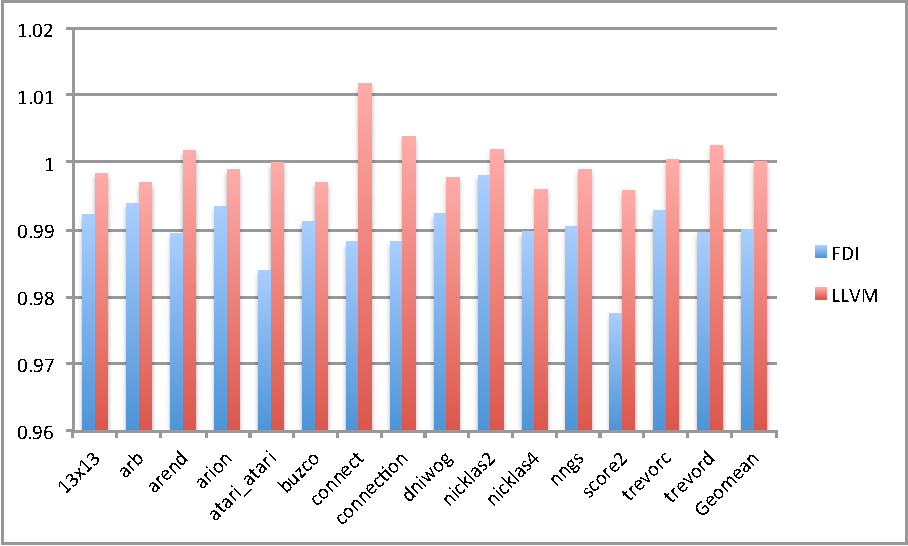
\includegraphics[width=1.00\linewidth]{Figures/speedupgbkall}
  \caption{Running times of the \gobmk\ inlined versions, normalized by Never}
  \label{fig:speedupgobmk}
\end{figure}


\subsection{Presenting the slowdown results}
\label{sec:slowdown}

Proceeding as described in \refSection{sec:description}, the data points for these experiments were selected as the worst-run times for \FDI\ and the best-run times for \llvm. This time the single-run experiments report a slowdown.

\subsubsection{Case Study 1 \gcc}

The slowdown over \llvm\ measured is of $2.43 \%$ for \gcc, as shown in \refTable{tab:slowdowngcc}. \refFigure{fig:WorstFDIBestLLVMgcc} shows the normalized running time for the slowdown measured for \gcc.

\begin{table}
  \centering
  \begin{tiny}
  
\begin{tabular}{lllllll}

{\bf Input} & {\bf \FDO\ normalized} & {\bf \llvm\ normalized} & {\bf Speedup} \\ \hline

166 & 0.9755 & 0.9755 & 0.00\%  \\
200 & 0.9807 & 0.9594 & 2.17\%  \\
c-typeck & 0.9845 & 0.9845 & 0.00\%  \\
cccp & 0.9949 & 0.9646 & 3.05\%  \\
cp-decl & 0.9784 & 0.9784 & 0.00\%  \\
expr & 0.9686 & 0.9567 & 1.23\%  \\
expr2 & 0.9686 & 0.9686 & 0.00\%  \\
g23 & 1.0574 & 1.0441 & 1.26\%  \\
integrate & 1.0253 & 2.47\%  \\
s04 & 1.0420 & 1.0153 & 2.56\%  \\
scilab & 1.0281 & 0.9886 & 3.84\%  \\
bzipR-all & 1.0315 & 1.0055 & 2.52\%  \\
lbm-all & 1.0909 & 1.0303 & 5.56\%  \\
mcf-all & 1.108108 & 1.0270 & 7.32\%  \\
parser-all & 1.049839 & 1.0059 & 4.18\%  \\  \hline
Geomean & & & 2.43\% \\

\hline
\end{tabular}

  \end{tiny}
  \caption{Data reflecting a slowdown on \gcc}
  \label{tab:slowdowngcc}
\end{table}


\subsubsection{Case Study 2: \bzip\  and \gzip}

The slowdown over \llvm\ measured is of $0.71 \%$ for \bzip, $8.84 \%$ for \gzip, as shown in \refTable{tab:slowdownb}, \refTable{tab:slowdownz}.

\begin{table}
  \centering
  \begin{tiny}
  
\begin{tabular}{lllll}

{\bf Input} & {\bf Normalized \FDO} & {\bf Normalized \llvm} & {\bf Slowdown} \\ \hline

auriel & 0.9961 & 1.0025 & 0.9936  \\ 
cards & 1.0457 & 0.9882 & 1.0581  \\
ocal & 1.0035 & 0.9984 & 1.0051  \\ 
proteins-2 & 1.0012 & 0.9931 & 1.0080  \\
revelation & 1.0359 & 0.9905 & 1.0458  \\  \hline
Geomean & & & 1.0218 \\

\hline
\end{tabular}

  \end{tiny}
  \caption{Data reflecting a slowdown on \bzip}
  \label{tab:slowdownb}
\end{table}

\begin{table}
  \centering
  \begin{tiny}
  
\begin{tabular}{lllllll}

{\bf Input} & {\bf Normalized \FDO} & {\bf Normalized \llvm} & {\bf Slowdown} \\ \hline

avernum & 1.0093 & 1.0062 & 0.31\%  \\
cards & 1.0092 & 1.0092 & 0.00\%  \\
ebooks & 1.0081 & 1.0081 & 0.00\%  \\
potemkin-mp4 & 1.0052 & 1.0079 & -0.26\%  \\
proteins-1 & 1.0203 & 1.0064 & 1.37\%  \\
revelation-ogg & 1.0072 & 1.0072 & 0.00\%  \\
usrlib-so & 1.0651 & 1.0016 & 5.96\%  \\
auriel & 1.1363 & 0.9924 & 2.67\%  \\
gcc-453 & 1.1111 & 1.0085 & 9.23\%  \\
lib-a & 1.0735 & 1.0151 & 5.44\%  \\
mohicans-ogv & 1.2835 & 0.9269 & 27.78\%  \\
ocal-019 & 1.1412 & 1.0122 & 11.31\%  \\
paintings-jpg & 1.1826 & 0.9561 & 19.15\%  \\
proteins-2 & 1.0780 & 1.0074 & 6.55\%  \\
sherlock-mp3 & 1.2692 & 0.9411 & 25.85\%  \\  \hline
Geomean & & & 8.84\% \\

\hline
\end{tabular}

  \end{tiny}
  \caption{Data reflecting a slowdown on \gzip}
  \label{tab:slowdownz}
\end{table}

\subsubsection{Case Study 3: \gobmk}

The slowdown over \llvm\ measured is of $0.99 \%$ for \gobmk, as shown in \refTable{tab:slowdowngobmk}.

\begin{table}
  \centering
  \begin{tiny}
  
\begin{tabular}{lllllll}

{\bf Input} & {\bf \FDO\ normalized} & {\bf \llvm\ normalized} & {\bf Speedup} \\ \hline

arend & 1.0111 & 1.0019 & 1.0091  \\
atari\_atari & 1.0000 & 	0.9892 & 1.0108  \\
connect & 1.0177 & 1.0059 & 1.0117  \\
connection & 1.0078 & 1.0039 & 1.0039  \\
nngs & 1.0123 & 0.9984 & 1.0138  \\
score2 & 1.0044 & 0.9960 & 1.0084  \\
trevord & 1.0078 & 1.0030 & 1.0048  \\   \hline
Geomean & & & 1.0089 (0.89 \%) \\

\hline
\end{tabular}

  \end{tiny}
  \caption{Data reflecting a slowdown on \gobmk}
  \label{tab:slowdowngobmk}
\end{table}
